% Editable vector artwork for the JSS manuscript.
% Rebuild from manuscript/jss/ with the configured TeX Live binary:
% pdflatex -interaction=nonstopmode -halt-on-error \
%   -output-directory=figures figures/framework_s1_s2_m1.tex
% The resulting PDF is included at text width; no raster assets are used.
\documentclass[tikz,border=2pt]{standalone}
\usepackage[T1]{fontenc}
\usepackage{amsmath}
\usetikzlibrary{arrows.meta}
\renewcommand{\familydefault}{\sfdefault}

\begin{document}
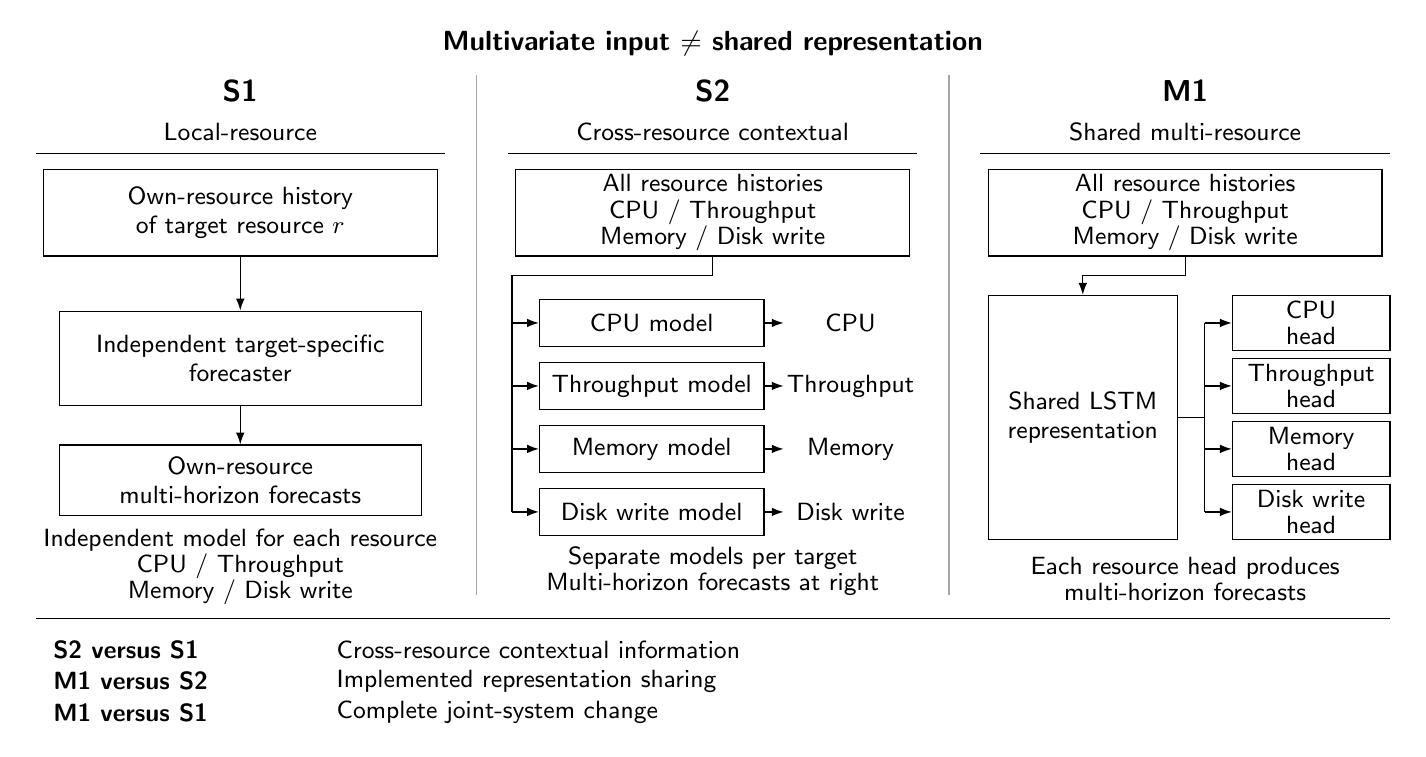
\begin{tikzpicture}[
  x=1mm,y=1mm,
  font=\fontsize{9}{10.5}\selectfont,
  line width=0.45pt,
  flow/.style={-{Latex[length=1.5mm,width=1.1mm]}},
  box/.style={draw,rectangle,align=center,inner sep=1.5pt},
  heading/.style={font=\fontsize{11}{12}\selectfont\bfseries},
  smalllabel/.style={font=\fontsize{9}{9.5}\selectfont,align=center},
  pair/.style={anchor=west,font=\fontsize{9}{10.5}\selectfont\bfseries}
]
  % Fixed geometry keeps the three formulations horizontally aligned.
  \path[use as bounding box] (0,-16) rectangle (174,73);
  \node[font=\fontsize{10}{11}\selectfont\bfseries] at (87,71)
    {Multivariate input $\neq$ shared representation};

  \node[heading] at (27,65) {S1};
  \node[heading] at (87,65) {S2};
  \node[heading] at (147,65) {M1};
  \node at (27,59.8) {Local-resource};
  \node at (87,59.8) {Cross-resource contextual};
  \node at (147,59.8) {Shared multi-resource};
  \draw (1,57) -- (53,57);
  \draw (61,57) -- (113,57);
  \draw (121,57) -- (173,57);
  \draw[black!35] (57,1) -- (57,67);
  \draw[black!35] (117,1) -- (117,67);

  % S1: one compact pipeline, explicitly repeated independently per resource.
  \node[box,minimum width=50mm,minimum height=11mm] (s1input) at (27,49.5)
    {Own-resource history\\of target resource $r$};
  \node[box,minimum width=46mm,minimum height=12mm] (s1model) at (27,31)
    {Independent target-specific\\forecaster};
  \node[box,minimum width=46mm,minimum height=9mm] (s1output) at (27,15.5)
    {Own-resource\\multi-horizon forecasts};
  \draw[flow] (s1input.south) -- (s1model.north);
  \draw[flow] (s1model.south) -- (s1output.north);
  \node[smalllabel] at (27,4.5)
    {Independent model for each resource\\CPU / Throughput\\Memory / Disk write};

  % S2 and M1 have intentionally identical all-resource history boxes.
  \node[box,minimum width=50mm,minimum height=11mm,smalllabel] (s2input) at (87,49.5)
    {All resource histories\\CPU / Throughput\\Memory / Disk write};
  \node[box,minimum width=50mm,minimum height=11mm,smalllabel] (m1input) at (147,49.5)
    {All resource histories\\CPU / Throughput\\Memory / Disk write};

  % S2 input fan-out is only wiring: four disjoint target models follow it.
  \draw (s2input.south) -- (87,41.5) -- (61.5,41.5) -- (61.5,11.5);
  \foreach \resource/\level in {CPU/35.5,Throughput/27.5,Memory/19.5,Disk write/11.5} {
    \node[box,minimum width=28.5mm,minimum height=6mm] (model) at (79.25,\level)
      {\resource\ model};
    \draw[flow] (61.5,\level) -- (model.west);
    \draw[flow] (model.east) -- (96,\level);
    \node[smalllabel,text width=18.5mm] at (104.5,\level) {\resource};
  }
  \node[smalllabel] at (87,4)
    {Separate models per target\\Multi-horizon forecasts at right};

  % M1 has one shared LSTM feeding resource-specific output heads.
  \node[box,minimum width=24mm,minimum height=31mm] (shared) at (134,23.5)
    {Shared LSTM\\representation};
  \draw[flow] (m1input.south) -- (147,41.5) -- (134,41.5) -- (shared.north);
  \draw (shared.east) -- (149.5,23.5);
  \draw (149.5,11.5) -- (149.5,35.5);
  \foreach \resource/\level in {CPU/35.5,Throughput/27.5,Memory/19.5,Disk write/11.5} {
    \node[box,minimum width=20mm,minimum height=7mm,smalllabel] (head) at (163,\level)
      {\resource\\head};
    \draw[flow] (149.5,\level) -- (head.west);
  }
  \node[smalllabel] at (147,3)
    {Each resource head produces\\multi-horizon forecasts};

  % A comparison band names contrasts without arithmetic or gain values.
  \draw (1,-2) -- (173,-2);
  \node[pair] at (2,-6) {S2 versus S1};
  \node[anchor=west] at (38,-6) {Cross-resource contextual information};
  \node[pair] at (2,-10) {M1 versus S2};
  \node[anchor=west] at (38,-10) {Implemented representation sharing};
  \node[pair] at (2,-14) {M1 versus S1};
  \node[anchor=west] at (38,-14) {Complete joint-system change};
\end{tikzpicture}
\end{document}
